\documentclass[tikz,border=2pt,11pt]{standalone}
\usetikzlibrary{arrows.meta}
\usetikzlibrary{calc}
\usetikzlibrary{fit}
\usetikzlibrary{positioning}
\usepackage{amsmath}
\usepackage{amssymb}
\usepackage{tikz}
\usepackage{xcolor}
\newcommand{\R}{\mathbb{R}}
\newcommand{\Z}{\mathbb{Z}}
\newcommand{\N}{\mathbb{N}}
\newcommand{\E}{\mathbb{E}}
\newcommand{\Pp}{\mathbb{P}}
\newcommand{\one}{\mathbf{1}}
\newcommand{\eps}{\varepsilon}
\newcommand{\norm}[1]{\lVert#1\rVert}
\newcommand{\abs}[1]{\lvert#1\rvert}
\DeclareMathOperator{\Var}{Var}
\DeclareMathOperator{\TV}{TV}
\DeclareMathOperator{\diag}{diag}
\DeclareMathOperator{\vol}{vol}
\DeclareMathOperator{\supp}{supp}
\begin{document}
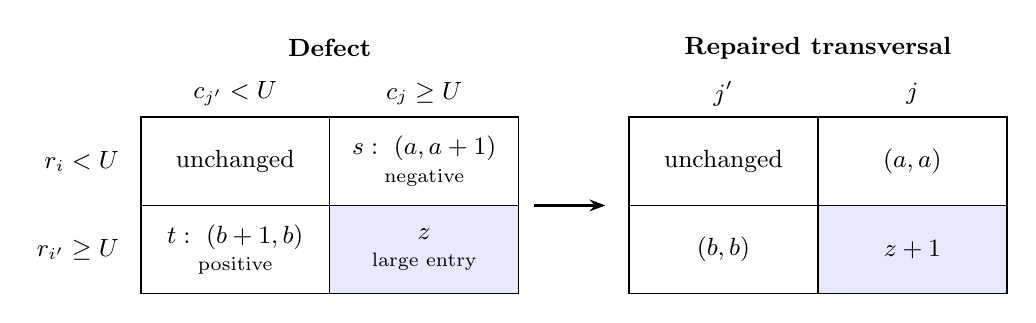
\begin{tikzpicture}[x=1cm,y=1cm,font=\small,
 cell/.style={minimum width=2.4cm,minimum height=1.12cm,inner sep=1pt},
 every path/.style={line width=.55pt}]
 \begin{scope}
  \fill[blue!9] (2.4,-2.24) rectangle (4.8,-1.12);
  \draw (0,0) rectangle (4.8,-2.24);
  \draw (2.4,0)--(2.4,-2.24);
  \draw (0,-1.12)--(4.8,-1.12);
  \node at (2.4,.88) {\textbf{Defect}};
  \node at (1.2,.3) {$c_{j'}<U$};
  \node at (3.6,.3) {$c_j\ge U$};
  \node[anchor=east] at (-.15,-.56) {$r_i<U$};
  \node[anchor=east] at (-.15,-1.68) {$r_{i'}\ge U$};
  \node[cell] at (1.2,-.56) {unchanged};
  \node[cell,align=center] at (3.6,-.56) {$s:\ (a,a+1)$\\[-1pt]\scriptsize negative};
  \node[cell,align=center] at (1.2,-1.68) {$t:\ (b+1,b)$\\[-1pt]\scriptsize positive};
  \node[cell,align=center] at (3.6,-1.68) {$z$\\[-1pt]\scriptsize large entry};
 \end{scope}
 \draw[-{Stealth[length=2mm]},thick] (5.0,-1.12)--(5.9,-1.12);
 \begin{scope}[xshift=6.2cm]
  \fill[blue!9] (2.4,-2.24) rectangle (4.8,-1.12);
  \draw (0,0) rectangle (4.8,-2.24);
  \draw (2.4,0)--(2.4,-2.24);
  \draw (0,-1.12)--(4.8,-1.12);
  \node at (2.4,.88) {\textbf{Repaired transversal}};
  \node at (1.2,.3) {$j'$};
  \node at (3.6,.3) {$j$};
  \node[cell] at (1.2,-.56) {unchanged};
  \node[cell] at (3.6,-.56) {$(a,a)$};
  \node[cell] at (1.2,-1.68) {$(b,b)$};
  \node[cell] at (3.6,-1.68) {$z+1$};
 \end{scope}
\end{tikzpicture}
\end{document}
